% Copyright Aidan Randle-Conde 2007-2014
% http://www.aidansean.com/phd_notes
% Anyone is free to download, redistribute, edit and use these notes and the source tex files with the following restrictions:
% This 
%  This message is included in the tex source files.
%  Aidan Randle-Conde is credited as the author.
%  Images are correctly credited to their respective authors, as outlined in the references.
%  No part of these notes may be used for commercial purposes.

\chapter{Relativistic spin\texorpdfstring{$-\frac{1}{2}$}{-1Over2} particles (Dirac equation)}
\chaptermark{Relativistic spin$-\frac{1}{2}$ particles}

\section{Non-relativistic description}

There are two spin states, up ($\frac{1}{2}$) and down ($-\frac{1}{2}$).  In spin space there are spin operators given by:

\[
  \bar{s} = \frac{\hbar}{2}\bar{\sigma}
\]

where $\bar{\sigma}$ are the so-called Pauli matrices.  The spin algebra is the same as that of orbital angular momentum.:

\[
  L^2 = l(l+1)\hbar^2
\]

In angular spin momentum:

\[
  S^2 = s(s+1)\hbar^2
\]

The Pauli matrices are:

\begin{eqnarray*}
  \bar{\sigma}_x & = &
  \left(
    \begin{array}{cc}
    0 & 1 \\
    1 & 0
    \end{array}
  \right)
  \\
  \bar{\sigma}_y & = &
  \left(
    \begin{array}{cc}
    0 & -i \\
    i & 0
    \end{array}
  \right)
  \\
  \bar{\sigma}_z & = &
  \left(
    \begin{array}{cc}
    1 & 0 \\
    0 & -1
    \end{array}
  \right)
  \\
  \textrm{where } \bar{I} & = & \bar{\sigma}_x^2 = \bar{\sigma}_y^2 = \bar{\sigma}_z^2
\end{eqnarray*}

The communtation relations are: \nopagebreak

\begin{eqnarray*}
  [\bar{s}_x,\bar{s}_y] & = & i\hbar \bar{s}_z \\
  \textrm{ie} \Bigg[ \frac{\hbar}{2}\bar{\sigma}_x,\frac{\hbar}{2}\bar{\sigma}_y \Bigg] & = & i\left(\frac{\hbar}{2}\right)^2\bar{\sigma}_z
\end{eqnarray*}

Or generally:

\[
  \Big[\bar{\sigma}_i,\bar{\sigma}_j\Big] = 2i\epsilon_{ijk}\bar{\sigma}_k
\]

where $\epsilon_{ijk}$ is the antisymmetric tensor.

\[
  \epsilon_{ijk} = 
  \Bigg\{
    \begin{array}{cc}
    0  & \textrm{if any index is repeated} \\
    1  & \textrm{for } 123, 231, 312 \\
    -1 & \textrm{for } 132, 321, 213
    \end{array}
\]

Also: $\bar{\sigma}_i\bar{\sigma}_j + \bar{\sigma}_j\bar{\sigma}_i = 2\delta_{ij}\bar{I}$.  This is the anticommutation relation.

\[
  \Rightarrow \bar{\sigma}_i\bar{\sigma}_j = \delta_{ij} \bar{I} + i\epsilon_{ijk}\bar{\sigma}_k
\]

\begin{eqnarray*}
  \textrm{Consider }\bar{\sigma}_i\ul{A}\bar{\sigma}_j\ul{B}_j & = & \ul{A}_i\ul{B}_j\delta_{ij} + i\epsilon_{ijk}\bar{\sigma}_k\ul{A}_i\ul{B}_j \\
  \textrm{then } \left(\bar{\sigma}\cdot\ul{A}\right)\left(\bar{\sigma}\cdot\ul{B}\right) & = & \ul{A}\cdot\ul{B} + i\bar{\sigma}\cdot\left(\ul{A}\times\ul{B}\right) \\
  & = & \ul{A}\cdot\ul{B} + i
  \Bigg|
    \begin{array}{ccc}
    \bar{\sigma}_x  & \bar{\sigma}_y  & \bar{\sigma}_z  \\
    \ul{A}_x & \ul{A}_y & \ul{A}_z \\
    \ul{B}_x & \ul{B}_y & \ul{B}_z
    \end{array}
  \Bigg|
\end{eqnarray*}

Suppose $\ul{A} = \ul{B} = \ul{p}$, then:

\[
  \left(\bar{\sigma}\cdot\ul{p}\right)\left(\bar{\sigma}\cdot\ul{p}\right) = |\ul{p}|^2
\]

The gyromagnetic ratio of a particle can be (correctly) determined if the expression for the energy is:

\[
  E = V + \frac{\left(\bar{\sigma}\cdot\ul{p}\right)\left(\bar{\sigma}\cdot\ul{p}\right)}{2m}
\]
as opposed to:
\[
  E = V + \frac{p^2}{2m}
\]
and the electromagnetic coupling is included.

Experimentally the gyromagnetically ratio is $g = 2.00232$ and the Dirac equation gives $g = 2$.

\section{The Dirac equation}

To avoid the problem of negative probability in the negative energy if the Klein-Gordon equation, Dirac proposed an equation linear in $\frac{\partial}{\partial t}$:

\[
  H\psi = \left(\bar{\alpha}\cdot\ul{p} + \beta m\right)\psi
\]

where $\bar{\alpha}$ and $\beta$ are $4\times 4$ matrices and solutions for $\psi$ are multi-component objects.  The formulation must be consistent with $E^2\psi = \left(p^2 + m^2\right)\psi$.

\begin{eqnarray*}
  \textrm{If } E\psi & = & \left(\alpha_ip_i + \beta m\right)\psi \\
  \textrm{then } E^2\psi & = & \left(\alpha_ip_i + \beta m\right)\left(\alpha_j p_j + \beta m\right)\psi \\
  & = & \left(\alpha_i\alpha_jp_ip_j + \left(\alpha_i\beta + \beta\alpha_j\right)p_im + \beta^2m^2\right)\psi \\
  & = & \left( \left(\frac{\alpha_i\alpha_j + \alpha_j\alpha_i}{2}p_ip_j + \alpha\left(\alpha_i\beta \beta\alpha_j\right)p_im + \beta^2m^2\right)\right)\psi \\
  \Rightarrow \bar{\alpha}_i\bar{\alpha}_j + \bar{\alpha}_j\bar{\alpha}_i & = & 2\delta_{ij}\bar{I} \\
  \bar{\alpha}\bar{\beta} + \bar{\beta}\bar{\alpha} & = & \bar{0} \\
  \bar{\beta}^2 & = & \bar{I}
\end{eqnarray*}

\begin{itemize}
  \item $\alpha$ and $\beta$ are Hermitian matrices: $\bar{\alpha} = \bar{\alpha}^{\dagger}$, $\bar{\beta} = \bar{\beta}^{\dagger}$.
  \item $\bar{\alpha}_i^2 = \bar{I}$
  \item $\alpha$ and $\beta$ are traceless
\end{itemize}

The proof that $\alpha$ and $\beta$ are traceless is as follows:

\[
  \bar{\alpha}_i\bar{\beta} = -\bar{\beta}\bar{\alpha}_i
\]

Postmultiplying by $\bar{\beta}$ gives:

\begin{eqnarray*}
  \bar{\alpha}_i\bar{\beta}^2 & = & -\bar{\beta}\bar{\alpha}_i\bar{\beta} \\
  \bar{\alpha}_i\bar{I} & = & -\bar{\beta}\bar{\alpha}_i\bar{\beta}
\end{eqnarray*}

Taking the trace:

\[
  Tr\left(\bar{\alpha}_i\right) = -Tr\left(\bar{\beta}\bar{\alpha}_i\bar{\beta}\right)
\]

Moving the elements cyclically:

\begin{eqnarray*}
  Tr\left(\bar{\alpha}_i\right) & = & - Tr\left(\bar{\beta}^2\bar{\alpha}_i\right) \\
  & = & - Tr\left(\bar{\alpha}_i\right) \\
  \textrm{So } Tr\left(\bar{\alpha}_i\right) & = & 0
\end{eqnarray*}

A common choice for $\bar{\alpha}$ and $\bar{\beta}$ is:

\begin{eqnarray*}
  \bar{\alpha}_i & = &
  \left(
    \begin{array}{cc}
    0 & \bar{\sigma}_i \\
    \bar{\sigma}_i & 0
    \end{array}
  \right)
  \\
  \bar{\beta} & = &
  \left(
    \begin{array}{cc}
    \bar{I} & 0 \\
    0 & -\bar{I}
    \end{array}
  \right)
\end{eqnarray*}

where $\bar{\sigma}_i$ are the Pauli matrices and $\bar{I}$ is the identity matrix.

\subsection{The covariant form of the Dirac equation}

\begin{eqnarray*}
  E\psi & = & \left(\bar{\alpha}_i\cdot\ul{p} + \beta m\right) \psi \\
  E & \to & i\frac{\partial}{\partial t} \\
  \ul{p} & \to & -i\ul{\nabla} \\
  \Rightarrow i\frac{\partial}{\partial t}\psi & = & -i \bar{\alpha}\cdot\ul{\nabla}\psi + \beta m\psi \\
\end{eqnarray*}

Premultiplying by $\beta$:

\begin{eqnarray*}
  i\beta \frac{\partial \psi}{\partial t} & = & -i\beta\bar{\alpha}\cdot\ul{\nabla}\psi + \beta^2 m \psi \\
  \textrm{So } i\beta\frac{\partial \psi}{\partial t} & = & -i\beta\bar{\alpha}\cdot\ul{\nabla}\psi + m\psi \\
  \textrm{Let } \gamma^0 & = & \beta \\
  \gamma^k & = & \beta\alpha \\
  i\gamma^0 \frac{\partial \psi}{\partial t} + i\gamma^k \ul{\nabla}\psi - m\psi & = & 0 \\
  \left( i\gamma^0 \frac{\partial}{\partial x^0} + i\gamma^k\frac{\partial}{\partial x^k} - m\right) & = & 0 \\
  \left( i\gamma^{\mu}\partial_{\mu} - m \right)\psi & = & 0 \\
  \textrm{where } \gamma^{\mu} & = & \left( \gamma^0,\ul{\gamma}^k\right) \\
  \partial_{\mu} & = & \left( \frac{\partial}{\partial x^0},\ul{\nabla}\right)
\end{eqnarray*}

$\gamma^0$ is Hermitian, since $\beta$ is Hermitian.  However, $\gamma^k$ is not Hermitian:

\begin{eqnarray*}
  \left(\gamma^k\right)^{\dagger} & = & -\gamma^k \\
  \gamma^k & = & \beta\alpha^k \\
  \left(\gamma\right)^{\dagger} & = & \left(\beta \alpha^k \right)^{\dagger} \\
  & = & \left(\alpha^k\right)^{\dagger}\beta^{\dagger} \\
  & = & \alpha^k\beta \\
  & = & -\beta\alpha^k \\
  & = & -\gamma^k
\end{eqnarray*}

\[
  \left(\gamma^0\right)^2 = \bar{I} \textrm{ as } \beta^2 = \bar{I}
\]

\begin{eqnarray*}
  \left(\gamma^k\right)^2 & = & \gamma^k\gamma^k \\
  & = & \beta\alpha^k\beta\alpha^k \\
  & = & -\beta\alpha^k\alpha^k\beta \\
  & = & -\beta\beta \\
  & = & -I
\end{eqnarray*}

\subsection{Adjoint Dirac equation and conserved current}

Since the Dirac equation is a matrix equation, to obtain the adjoint equation it is necessary to take the Hermitian conjugate and not the complex conjugate.

\begin{eqnarray}
  \left(i\gamma^{\mu}\partial_{\mu} -m \right)\psi & = & 0 \label{eq:dirac} \\
  \textrm{or } \left( i\gamma^0\frac{\partial}{\partial t} + i\gamma^k\frac{\partial}{\partial x^k} - m \right)\psi & = & 0 \nonumber
\end{eqnarray}

Taking the Hermitian conjugate:

\[
  -i\frac{\partial \psi^{\dagger}}{\partial t}\gamma^0 - i\frac{\partial \psi^{\dagger}}{\partial x^k}\left(-\gamma^k\right) - m\psi^{\dagger} = 0
\]

Postmultiply by $\gamma^0$:

\begin{eqnarray*}
  -i\frac{\partial \psi^{\dagger}}{\partial t} + i\frac{\partial \psi^{\dagger}}{\partial x^k}\gamma^k\gamma^0 - m\psi^{\dagger}\gamma^0 & = & 0 \\
  \gamma^0\gamma^k & = & -\gamma^k\gamma^0 \\
  \Rightarrow -i\frac{\partial \psi^{\dagger}}{\partial t} - i\frac{\partial \psi^{\dagger}}{\partial x^k}\gamma^0\gamma^k - m\psi^{\dagger}\gamma^0 & = & 0
\end{eqnarray*}

Defining the adjoint as:

\[
  \bar{\psi} = \psi^{\dagger}\gamma^0
\]

gives: \nopagebreak

\begin{eqnarray}
  -i \frac{\partial \bar{\psi}}{\partial t}\gamma^0 - i \frac{\partial \bar{\psi}}{\partial x^k}\gamma^k -m\bar{\psi} & = & 0 \nonumber \\
  \textrm{or } i\partial_{\mu}\bar{\psi}\gamma^{\mu} + m\bar{\psi} & = & 0 \label{eq:adjointdirac}
\end{eqnarray}
  
Consider $\bar{\psi}\times$(\ref{eq:dirac})$+$(\ref{eq:adjointdirac})$\times\psi$:

\begin{eqnarray*}
  \bar{\psi}\times(\ref{eq:dirac}) & = & \bar{\psi}i\gamma^{\mu}\partial_{\mu}\psi - \bar{\psi}m\psi = 0 \\
  (\ref{eq:adjointdirac})\times\psi & = & i\partial_{\mu}\bar{\psi}\gamma^{\mu}\psi + m\bar{\psi}\psi = 0 \\
  \textrm{So } i\bar{\psi}\gamma^{\mu}\partial_{\mu}\psi + i\partial_{\mu}\bar{\psi}\gamma^{\mu}\psi & = & 0 \\
  \Rightarrow \partial_{\mu} \left(\bar{\psi}\gamma^{\mu}\psi\right) & = & 0
\end{eqnarray*}

So the expression for $j^{\mu}$:

\[
  j^{\mu} = \bar{\psi}\gamma^{\mu}\psi
\]

satisfies the continuity equation.

$j^{\mu}$ is identified as the probability and flux densities $\rho$ and $\ul{j}$.

The probability density is:

\begin{eqnarray*}
  \rho & = & j^0 \\
  & = & \bar{\psi}\psi \\
  & = & \psi^{\dagger}\gamma^0\gamma^0\psi \\
  & = & \psi^{\dagger}\psi \\
  & = & |\psi|^2
\end{eqnarray*}

Hence $\rho$ is always positive.  For the electromagnetic interaction the charge current density is:

\[
  j^{\mu} = -\e\bar{\psi}\gamma^{\mu}\psi
\]

\subsection{Free particle solutions of the Dirac equation}

Consider solutions of the form:

\[
  \psi = u(p)\e^{-ipx}
\]

Substitute $\psi$ into the Dirac equation:

\begin{eqnarray*}
  \left(i\gamma^{\mu}\partial_{\mu} - m\right)u(p)\e^{-ipx} & = & 0 \\
  \left(i\gamma^{\mu}\left(-ip_{\mu}\right)-m\right)u(p)\e^{-ipx} & = & 0 \\
  \left(\gamma^{\mu}p_{\mu} - m\right)u(p)\e^{-ipx} & = & 0 \\
  \textrm{So } \left(\gamma^{\mu}p_{\mu}-m\right)u(p) & = & 0 \\
  \textrm{Define } \gamma^{\mu}p_{\mu} & = & \not{p} \\
  \textrm{So } \left(\not{p} - m\right)u(p) & = & 0
\end{eqnarray*}

To obtain solutions for $u(p)$, write the above in terms of the $\alpha$ and $\beta$ matrices:

\[
  \left(\gamma^0E - \gamma^kp_k - m\right)u(p) = 0
\]

Premultiplying by $\gamma^0$:

\begin{eqnarray*}
  \left(\left(\gamma^0\right)^2E - \gamma^0\gamma^kp_k - \gamma^0m\right)u(p) & = & 0 \\
  \left(IE - \alpha^kp_k -\beta m\right) u(p) & = & 0
\end{eqnarray*}

For a particle at rest, $\ul{p} = \ul{0}$:

\begin{eqnarray*}
  \left(IE - \beta m\right)u(p) & = & 0 \\
  \Rightarrow m
  \left(
    \begin{array}{cc}
    I & 0 \\
    0 & -I
    \end{array}
  \right)
  u(p)
  & = & 
  \left(
    \begin{array}{cc}
    I & 0 \\
    0 & I
    \end{array}
  \right)
  Eu(p)
\end{eqnarray*}

Solutions exist if:

\[
  \Bigg|
    \begin{array}{cc}
    (m - E)I & 0 \\
    0 & -(m + E)I
    \end{array}
  \Bigg|
  = 0
\]

or in longhand:

\begin{eqnarray*}
  \left|
    \begin{array}{cccc}
    m-E & 0 & 0 & 0  \\
    0 & m-E & 0 & 0  \\
    0 & 0 & -m-E & 0 \\
    0 & 0 & 0 & -m-e
    \end{array}
  \right|
  & = & 0 \\
  \Big[\left(m-E\right)\left(m+E\right)\Big]^2 & = & 0
\end{eqnarray*}

So there are four eigenvalues corresponding to $E = \pm m$ in two coincident pairs.  This means that negative energy solutions still exist.  $u_1, u_2$ are associated with positive energy solutions and $u_3, u_4$ are associated with negative energy solutions.

Consider the solutions when $\ul{p} \neq \ul{0}$.  From $\left(\bar{\alpha}\cdot\ul{p} + \beta m\right)u = 0$:

\[
  \Bigg[
  \left(
    \begin{array}{cc}
    0 & \sigma \\
    \sigma & 0
    \end{array}
  \right)
  \cdot \ul{p}
  +
  \left(
    \begin{array}{cc}
    I & 0 \\
    0 & -I
    \end{array}
  \right)
  m
  \Bigg]
  \left(
    \begin{array}{c}
    u_A \\
    u_B
    \end{array}
  \right)
  = E
  \left(
    \begin{array}{c}
    u_A \\
    u_B
    \end{array}
  \right)
\]

This yields:

\begin{eqnarray}
  \bar{\sigma}\cdot\ul{p} u_B + mu_A & = & Eu_A \label{eq:diracub} \\
  \bar{\sigma}\cdot\ul{p} u_A - mu_B & = & Eu_B \label{eq:diracua}
\end{eqnarray}

\begin{eqnarray*}
  \textrm{From (\ref{eq:diracub}) } & u_A & = \frac{\bar{\sigma}\cdot\ul{p}u_B}{E - m} \\
  \textrm{From (\ref{eq:diracua}) } & u_A & = \frac{\bar{\sigma}\cdot\ul{p}u_A}{E + m}
\end{eqnarray*}

\begin{eqnarray*}
  \textrm{For } E>0: && \\
  u_A & =
  \left(
    \begin{array}{c}
    1 \\
    0
    \end{array}
  \right)
  & \textrm{ (spin up)}
  \\
  \textrm{or} && \\
  u_A & =
  \left(
    \begin{array}{c}
    0 \\
    1
    \end{array}
  \right)
  & \textrm{ (spin down)}
\end{eqnarray*}

\begin{eqnarray*}
  \textrm{So } u_1 & = & N
  \left(
    \begin{array}{c}
    1 \\
    0 \\
    \frac{\bar{\sigma}\cdot\ul{p}}{E + m} \\
    0
    \end{array}
  \right)
  \\
  u_2 & = & N
  \left(
    \begin{array}{c}
    0 \\
    1 \\
    0 \\
    \frac{\bar{\sigma}\cdot\ul{p}}{E + m}
    \end{array}
  \right)
\end{eqnarray*}

where $N$ is a normalisation constant.

For $E<0$:

\begin{eqnarray*}
  u_A & = & \frac{\bar{\sigma}\cdot\ul{p}}{E - m}u_B \\
  & = & \frac{\bar{\sigma}\cdot\ul{p}}{-|E| - m}u_B \\
  & = & -\frac{\bar{\sigma}\cdot\ul{p}}{|E| + m}u_B
\end{eqnarray*}

\begin{eqnarray*}
  \textrm{So } u_3 & = & N
  \left(
    \begin{array}{c}
    -\frac{\bar{\sigma}\cdot\ul{p}}{|E| + m} \\
    0 \\
    1 \\
    0
    \end{array}
  \right)
  \\
  u_4 & = & N
  \left(
    \begin{array}{c}
    0 \\
    -\frac{\bar{\sigma}\cdot\ul{p}}{E + m} \\
    0 \\
    1
    \end{array}
  \right)
\end{eqnarray*}

In summary all the above comes from:

\[
  \left( \not{p} - m \right) = 0
\]

with the propagation factor $\e^{-ipx}$.

Now associate negative energy solutions ($u_3,u_4$) such that they describe positron solutions propagating backwards in time with the propagation factor $\e^{ipx}$:

\begin{eqnarray*}
  u^{(3,4)}(-p)\e^{-i(-p)x} & = v^{(2,1)}(p)\e^{ipx} \\
  \Rightarrow v_2 & =
  \left(
    \begin{array}{c}
    \frac{\bar{\sigma}\cdot\ul{p}}{E + m} \\
    0 \\
    1 \\
    0
    \end{array}
  \right)
  & \textrm{ (spin down)}
  \\
  v_1 & =
  \left(
    \begin{array}{c}
    0 \\
    \frac{\bar{\sigma}\cdot\ul{p}}{E + m} \\
    0 \\
    1
    \end{array}
  \right)
  & \textrm{ (spin up)}
\end{eqnarray*}

The original equation for an electron of energy $-E$ and momentum $-\ul{p}$ is:

\begin{eqnarray*}
  \left(-\not{p} - m\right)u(-p) & = & 0 \\
  \Rightarrow \left(\not{p} + m\right)v(p) & = & 0
\end{eqnarray*}

\subsection{Orthogonality and normalisation of spinors}

\begin{eqnarray*}
  \psi_1 & = & N
  \left(
    \begin{array}{c}
    1 \\
    0 \\
    \frac{\bar{\sigma}\cdot\ul{p}}{E + m} \\
    0
    \end{array}
  \right)
  \e^{-ipx}
  \\
  \psi_2 & = & N
  \left(
    \begin{array}{c}
    0 \\
    1 \\
    0 \\
    \frac{\bar{\sigma}\cdot\ul{p}}{E + m}
    \end{array}
  \right)
  \e^{-ipx}
\end{eqnarray*}

For orthogonality:

\begin{eqnarray*}
  \int \psi_1^{\dagger}\psi_2\mathrm{d}^3x & = & 0 \\
  \Rightarrow N^{\star}N\left(1 0 \frac{\left(\bar{\sigma}\cdot\ul{p}\right)^{\dagger}}{E + m} 0\right)
  \left(
    \begin{array}{c}
    0 \\
    1 \\
    0 \\
    \frac{\bar{\sigma}\cdot\ul{p}}{E + m} 
    \end{array}
  \right)
  & = & 0
\end{eqnarray*}

So $\psi_1$ and $\psi_2$ are orthogonal to each other.  Similarly $\psi_3$ and $\psi_4$ are orthogonal to each other.

In order to normalise to $2E$ particles in a volume $V$:

\begin{eqnarray*}
  \int \psi_1^{\dagger}\psi_1\mathrm{d}^3x & = & 2E \\
  \Rightarrow \int N^{\star}N\left( 1 \quad 0 \quad \left(\frac{\bar{\sigma}\cdot\ul{p}}{E + m}\right)^{\dagger} \quad 0 \right)
  \left(
    \begin{array}{c}
    1 \\
    0 \\
    \frac{\bar{\sigma}\cdot\ul{p}}{E + m} \\
    0
    \end{array}
  \right)
  \mathrm{d}^3x & = & 2E
  \\
  \Rightarrow \int N^{\star}N\Bigg[ 1 + \left( \frac{\bar{\sigma}\cdot\ul{p}}{E + m} \right)^2 \Bigg]\mathrm{d}^3x & = & 2E \\
  \textrm{where } \left(\bar{\sigma}\cdot\ul{p}\right)^{\dagger} & = & \bar{\sigma}\cdot\ul{p}
\end{eqnarray*}

\begin{eqnarray*}
  \bar{\sigma}_y & = &
  \left(
    \begin{array}{cc}
    0 & -i \\
    i & 0
    \end{array}
  \right)
  \\
  \Rightarrow
  \left(
  \bar{\sigma}_y\cdot\ul{p}_y\right)^2 & = &
  \left(
    \begin{array}{cc}
    0 & -ip_y \\
    ip_y & 0
    \end{array}
  \right)^2
  \\
  & = &
  \left(
    \begin{array}{cc}
    p_y^2 & 0 \\
    0 & p_y^2
    \end{array}
  \right)
  \\
  & = & p_y^2 \bar{I}
\end{eqnarray*}

\begin{eqnarray*}
  \textrm{So } \int N^{\star}N\left( 1 + \frac{p^2}{\left(E + m\right)^2}\right)\mathrm{d}^3x & = & 2E \\
  \Rightarrow N^{\star}N\left(\frac{\left(E + m\right)^2 + E^2 - m^2}{\left(E + m\right)^2}\right)\mathrm{d}^3x & = & 2E \\
  & = & \int N^{\star}N\frac{2E}{E + m}\mathrm{d}^3 x \\
  \textrm{So } \frac{N^{\star}NV}{E + m} & = & 1 \\
  \Rightarrow N & = & \sqrt{\frac{E + m}{V}}
\end{eqnarray*}

\subsection{Spin}

Neither the orbital angular momentum nor the spin angular momentum commute with the Dirac Hamiltonian, but $J = L + S$ does commute.  To find an operator other than $J$ that commutes with the Dirac Hamiltonian recall the Dirac equation:

\[
  H
  \left(
    \begin{array}{c}
    u_A \\
    u_B
    \end{array}
  \right)
  =
  \left(\bar{\alpha}\cdot\ul{p} + \beta m\right)
  \left(
    \begin{array}{c}
    u_A \\
    u_B
    \end{array}
  \right)
\]

$\bar{\alpha}\cdot\ul{p} + \beta m$ is the Dirac Hamiltonian.

\begin{eqnarray*}
  H
  \left(
    \begin{array}{c}
    u_A \\
    u_B
    \end{array}
  \right)
  & = &
  E
  \left(
    \begin{array}{c}
    u_A \\
    u_B
    \end{array}
  \right)
  \\
  & = &
  \left(
    \begin{array}{cc}
    m\bar{I} & \bar{\sigma}\cdot\ul{p}\bar{I} \\
    \bar{\sigma}\cdot\ul{p}\bar{I} & -m\bar{I}
    \end{array}
  \right)
  \left(
    \begin{array}{c}
    u_A \\
    u_B
    \end{array}
  \right)
\end{eqnarray*}

By inspection, the Dirac Hamiltonian commutes with $\bar{\sigma}\cdot\ul{p}\bar{I}$:

\[
\left(
  \begin{array}{cc}
  m\bar{I} & \bar{\sigma}\cdot\ul{p}\bar{I} \\
  \bar{\sigma}\cdot\ul{p}\bar{I} & -m\bar{I}
  \end{array}
\right)
\left(
  \begin{array}{cc}
  \bar{\sigma}\cdot\ul{p}\bar{I} & 0 \\
  0 & \bar{\sigma}\cdot\ul{p}\bar{I}
  \end{array}
\right)
  -
  \left(
    \begin{array}{cc}
    \bar{\sigma}\cdot\ul{p}\bar{I} & 0 \\
    0 & \bar{\sigma}\cdot\ul{p}\bar{I}
    \end{array}
  \right)
  \left(
    \begin{array}{cc}
    m\bar{I} & \bar{\sigma}\cdot\ul{p}\bar{I} \\
    \bar{\sigma}\cdot\ul{p}\bar{I} & m\bar{I}
    \end{array}
  \right)
  =
  \left(
    \begin{array}{cc}
    0 & 0 \\
    0 & 0
    \end{array}
  \right)
\]

Define the helicity operator as: 

\[
  H = \frac{1}{2}\bar{\sigma}\cdot\ul{\hat{p}} = \frac{1}{2} \frac{\bar{\sigma}\cdot\ul{p}}{|\ul{p}|}
\]

The helicity is the projection of the spin along the direction of motion and its eigenvalues are $\pm \frac{1}{2}$.  $H = \frac{1}{2}$ corresponds to positive helicity and $H = \frac{-1}{2}$ corresponds to negative helicity.

\begin{figure}[!htb]
  \begin{center}
    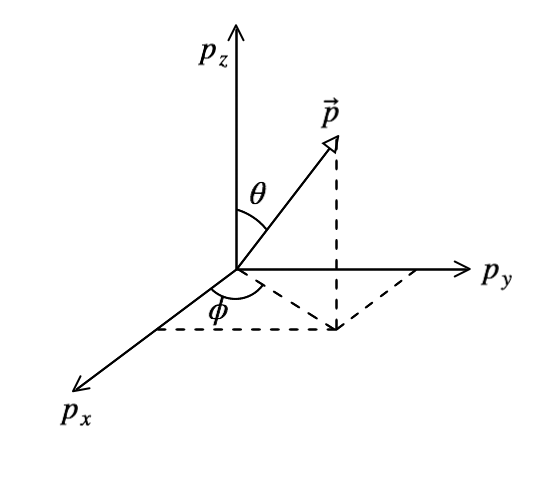
\includegraphics[width=0.75\textwidth]{images/web_feynman/image_24.png}
    \caption[Projection of momentum in three dimensions]{Projection of momentum in three dimensions.}
    \label{fig:ch8_momentum}
  \end{center}
\end{figure}

Suppose a particle has a momentum $\ul{p}$, with coordinates defined in figure \ref{fig:ch8_momentum}, where:

\begin{eqnarray*}
  \ul{\hat{p}} & = & \sin\theta\cos\phi\hat{\ul{i}} + \sin\theta\sin\phi\hat{\ul{j}} + \cos\theta\hat{\ul{k}} \\
  \bar{\sigma}\cdot\ul{\hat{p}} & = & \bar{\sigma}_x\cdot\ul{\hat{p}}_x + \bar{\sigma}_y\cdot\ul{\hat{p}}_y + \bar{\sigma}_z\cdot\ul{\hat{p}}_z \\
  & = &
  \left(
    \begin{array}{cc}
    0 & 1 \\
    1 & 0
    \end{array}
  \right)
  \sin\theta\cos\phi
  +
  \left(
    \begin{array}{cc}
    0 & -i \\
    i & 0
    \end{array}
  \right)
  \sin\theta\sin\phi
  +
  \left(
    \begin{array}{cc}
    1 & 0 \\
    0 & -1
    \end{array}
  \right)
  \cos\theta
  \\
  \textrm{So } \frac{1}{2}\bar{\sigma}\cdot\ul{\hat{p}}
  \left(
    \begin{array}{c}
    u_A \\
    u_B
    \end{array}
  \right)
  & = & \frac{1}{2}
  \left(
    \begin{array}{cc}
    \cos\theta & \sin\theta \e^{-i\phi} \\
    \sin\theta \e^{i\phi} & -\cos\theta
    \end{array}
  \right)
  \left(
    \begin{array}{c}
    u_A \\
    u_B
    \end{array}
  \right)
\end{eqnarray*}

So the eigenvalue equation is:

\begin{eqnarray*}
  \frac{1}{2}
  \left(
    \begin{array}{cc}
    \cos\theta & \sin\theta \e^{-i\phi} \\
    \sin\theta\e^{i\phi} & -\cos\theta
    \end{array}
  \right)
  \left(
    \begin{array}{c}
    u_A \\
    u_B
    \end{array}
  \right)
  & = & \lambda
  \left(
    \begin{array}{c}
    u_A \\
    u_B
    \end{array}
  \right)
  \\
  \Bigg|
    \begin{array}{cc}
    \cos\theta - 2\lambda & \sin\theta\e^{-i\phi} \\
    \sin\theta\e^{i\phi} & -\cos\theta - 2\lambda
    \end{array}
  \Bigg|
  & = & 0 \\
  \left(-\cos\theta-2\lambda\right)\left(\cos\theta+2\lambda\right) - \sin^2\theta & = & 0 \\
  -\cos^2\theta + 4\lambda^2 - \sin^2\theta & = & 0 \\
  \Rightarrow \lambda & = & \pm\frac{1}{2}
\end{eqnarray*}

\subsection{The \texorpdfstring{$\gamma^5$}{G5} matrix}

The $\gamma^5$ matrix is used to simplify notation:

\[
  \gamma^5 = i\gamma^0\gamma^1\gamma^2\gamma^3
\]

$\gamma^5$ has many properties:

\begin{eqnarray*}
  \left(\gamma^5\right)^{\dagger} & = & \gamma^5 \\
  \left(\gamma^5\right)^2 & = & \bar{I} \\
  \gamma^5\gamma^{\mu} + \gamma^{\mu}\gamma^5 & = & 0
\end{eqnarray*}

Ãn Dirac-Pauli representation:

\begin{eqnarray*}
  \gamma^0 & = &
  \left(
    \begin{array}{cc}
    \bar{I} & \bar{0} \\
    \bar{0} & \bar{I}
    \end{array}
  \right)
  \\
  \gamma^k & = &
  \left(
    \begin{array}{cc}
    \bar{0} & \bar{\sigma}_k \\
    \bar{\sigma}_k & \bar{0}
    \end{array}
  \right)
  \\
  \gamma^5 & = &
  \left(
    \begin{array}{cc}
    \bar{0} & \bar{I} \\
    \bar{I} & \bar{0}
    \end{array}
  \right)
\end{eqnarray*}

Consider the effect of $\gamma^5$ operating upon the Dirac equation (dropping the bars that signify matrices):

\begin{eqnarray*}
  \gamma^5
  \left(
    \begin{array}{c}
    u_A \\
    u_B
    \end{array}
  \right)
  & = &
  \left(
    \begin{array}{cc}
    0 & I \\
    I & 0
    \end{array}
  \right)
  \left(
    \begin{array}{c}
    \chi \\
    \left(\frac{\sigma\cdot p}{E + m}\right)\chi
    \end{array}
  \right)
  \\
  \textrm{where }\chi & = &
  \left(
    \begin{array}{c}
    1 \\
    0
    \end{array}
  \right)
  \\
  \gamma^5
  \left(
    \begin{array}{c}
    u_A \\
    u_B
    \end{array}
  \right)
  & = &
  \left(
    \begin{array}{c}
    \left(\frac{\sigma\cdot p}{E + m}\right)\chi \\
    \chi
    \end{array}
  \right)
\end{eqnarray*}

For high energies, or in the limit $m \to 0$, $E \sim p$:

\begin{eqnarray*}
  \gamma^5
  \left(
    \begin{array}{c}
    u_A \\
    u_B
    \end{array}
  \right)
  & \simeq &
  \left(
    \begin{array}{c}
    \sigma\cdot\hat{p} \chi \\
    \chi
    \end{array}
  \right)
  \\
  & = &
  \left(
    \begin{array}{c}
    \sigma\cdot\hat{p}\chi \\
    I\chi
    \end{array}
  \right)
  \\
  & = & 
  \left(
    \begin{array}{c}
    \sigma\cdot\hat{p}\chi \\
    \left(\sigma\cdot\hat{p}\right)^2\chi
    \end{array}
  \right)
  \\
  & = &
  \sigma\cdot\hat{p}
  \left(
    \begin{array}{c}
    \chi \\
    \sigma\cdot\hat{p}\chi
    \end{array}
  \right)
  \\
  & = &
  \sigma\cdot\hat{p}
  \left(
    \begin{array}{c}
      \chi \\
      \left(\frac{\sigma\cdot\ p}{E + m}\right)\chi
    \end{array}
  \right)
  \\
  & = &
  \sigma\cdot\hat{p}
  \left(
    \begin{array}{c}
    u_A \\
    u_B
    \end{array}
  \right)
  \\
  \textrm{So }\gamma^5
  \left(
    \begin{array}{c}
    u_A \\
    u_B
    \end{array}
  \right)
  & = &
  \left(
    \begin{array}{cc}
    \sigma\cdot\hat{p} & 0 \\
    0 & \sigma\cdot\hat{p}
    \end{array}
  \right)
  \left(
    \begin{array}{c}
    u_A \\
    u_B
    \end{array}
  \right)
\end{eqnarray*}

So in the limit $m \to 0$, $\gamma^5$ becomes the helicity operator.

Operators can then be defined as follows:

\begin{eqnarray*}
  P_R & = & \frac{1}{2}\left(1 + \gamma^5\right) \\
  P_L & = & \frac{1}{2}\left(1 - \gamma^5\right)
\end{eqnarray*}

These operators are then respectively the left and right-handed projection operators of helicity.

Where $m\neq 0$ (which is generally the case) the operator $\frac{1}{2}\left(1 + \gamma^5\right)$ is the right-handed chirality state and if $m$ is small then the state can be approximated as a right-handed helicity state, but will also contain a small fraction of the left-handed helicity component.

\subsection{Completeness relation}

The completeness relations are used extensively in the evaluation of Feynmann diagram calculations.

Consider the summation over all spin states:

\begin{eqnarray*}
  \sum_{S = 1,2} u_s(p)\bar{u}_s(p) & = &  \sum_{S = 1,2} N^{\star}N
  \left(
    \begin{array}{c}
    \chi_S \\
    \frac{\sigma \cdot p}{E + m}\chi_S
    \end{array}
  \right)
  \left( \chi_S^{\dagger} , -\frac{\sigma\cdot p}{E + m}\chi^{\dagger} \right) \\
  & = & \sum_{S = 1,2} N^{\star}N
  \left(
    \begin{array}{cc}
    \chi_S^{\dagger}\chi & -\frac{\left(\sigma\cdot p\right)^{\dagger}}{E + m}\chi_S^{\dagger}\chi_S \\
    \frac{\sigma\cdot p}{E + m}\chi_S^{\dagger}\chi_S & -\frac{E^2 - m^2}{\left(E + m\right)^2}\chi_S^{\dagger}\chi_S
    \end{array}
  \right)
  \\
  & = & \sum_{S = 1,2}N^{\star}N
  \left(
    \begin{array}{cc}
    I & -\frac{\left(\sigma\cdot p\right)^{\dagger}}{E + m} \\
    \frac{\sigma\cdot p}{E + m} & -\frac{E^2 - m^2}{\left(E + m\right)^2}
    \end{array}
  \right)
  \chi_S^{\dagger}\chi
\end{eqnarray*}

The summation over states is:

\begin{eqnarray*}
  \sum_{S = 1,2} \chi_S^{\dagger}\chi_S & = &
  \left(
    \begin{array}{c}
    1 \\
    0
    \end{array}
  \right)
  \left(1 0\right)
  +
  \left(
    \begin{array}{c}
    0 \\
    1
    \end{array}
  \right)
  \left(0 1\right)
  \\
  & = &
  \left(
    \begin{array}{cc}
    1 & 0 \\
    0 & 1
    \end{array}
  \right)
\end{eqnarray*}

\[
  N^{\star}N = E + m
\]

\begin{eqnarray}
  \sum_{S = 1,2} u_S\bar{u}_S & = &
  \left(
    \begin{array}{cc}
    I & -\frac{\sigma\cdot p}{E + m} \\
    \frac{\sigma \cdot p}{E + m} & -\frac{E^2 - m^2}{\left(E + m\right)^2}I
    \end{array}
  \right)
  \left(E + m\right)
  \nonumber
  \\
  & = &
  \left(
    \begin{array}{cc}
    \left(E + m\right)I & -\sigma\cdot p \\
    \sigma\cdot p & -I\left(E - m\right)
    \end{array}
  \right)
  \nonumber
  \\
  & = &
  \left(
    \begin{array}{cc}
    \left(E + m\right)I & -\sigma\cdot p \\
    \sigma\cdot p & \left(m - E\right)I
    \end{array}
  \right)
  \label{eq:completeness1}
  \\
  \textrm{However } \not{p} + m & = & \gamma^{\mu}p_{\mu} + mI \nonumber \\
  & = & \gamma^0E - \gamma^kp_k + mI \nonumber \\
  & = &
  \left(
    \begin{array}{cc}
    I & 0 \\
    0 & -I
    \end{array}
  \right)
  E -
  \left(
    \begin{array}{cc}
    0 & \sigma_k \\
    -\sigma_k & 0
    \end{array}
  \right)
  p_k +
  \left(
    \begin{array}{cc}
    I & 0 \\
    0 & I
    \end{array}
  \right)
  m
  \nonumber
  \\
  & = &
  \left(
    \begin{array}{cc}
    \left(E + m\right) I & -\sigma\cdot p \\
    \sigma\cdot p & \left(m - E\right) I
    \end{array}
  \right)
  \label{eq:completeness2}
\end{eqnarray}

So (\ref{eq:completeness1})$ = $(\ref{eq:completeness2}).

\begin{eqnarray*}
  \sum_{S = 1,2} u_S\bar{u}_S & = & \not{p} + m \\
  \sum_{S = 1,2} v_S\bar{v}_S & = & \not{p} - m
\end{eqnarray*}

\subsection{Possible forms of interaction}

An exhasutive set of possibilities of interaction is:

\paragraph*{Scalar interactions} $\bar{u}u$ (even parity)
\paragraph*{Vector interactions} $\bar{u}\gamma^{\mu}u$ (odd parity)  This interaction causes allowed Fermi transitions in $\beta$ decay and in $\mu$ decay.  
\paragraph*{Tensor interactions} $\bar{u}\sigma^{\mu\nu}u$  As far as has been confirmed by experiment this interaction does not exist, except for anomalous magnetic moments.
\paragraph*{Axial vector interactions} $\bar{u}\gamma^5\gamma^{\mu}u$ (even parity)  The weak interaction is a mixture of the vector and axial vector interactions.  In some nuclei, either the vector or axial vector process cannot take place.  In many $\beta$ decays of nuclei both of the processes take place.
\paragraph*{Pseudoscalar interactions} $\bar{u}\gamma^5u$ (odd parity)

\section{Trace theorems}

\subsection{\texorpdfstring{$Tr[I]$}{TrI}}

\[
  Tr[I] = 4
\]

\subsection{\texorpdfstring{$Tr[\not{a}\not{b}]$}{TrNotANotB}}

\begin{eqnarray*}
  Tr[\not{a}\not{b}] & = & Tr[\not{b}\not{a}] \\
  \textrm{So } Tr[\not{a}\not{b}] & = & \frac{1}{2}Tr[\not{a}\not{b} + \not{b}\not{a}] \\
  & = & \frac{1}{2} Tr[\gamma^{\mu}\gamma^{\nu}a_{\mu}b_{\nu} + \gamma^{\mu}\gamma^{\nu}b_{\mu}a_{\nu}] \\
  \gamma^{\mu}\gamma{^\nu} + \gamma^{\nu}\gamma^{\mu} & = & 2g^{\mu\nu}I \\
  & = & \frac{1}{2}a\cdot b 2 Tr[I] \\
  & = & 4a\cdot b
\end{eqnarray*}

\subsection{\texorpdfstring{$Tr[\not{a}\not{b}\not{c}\not{d}]$}{TrNotANotBNotCNotD}}

\begin{eqnarray*}
  Tr[\not{a}\not{b}\not{c}\not{d}] & = & Tr[\gamma^{\mu}\gamma^{\nu}\gamma^{\delta}\gamma^{\sigma}a_{\mu}b_{\nu}c_{\delta}d_{\sigma}] \\
  \textrm{But } Tr[\gamma^{\mu}\gamma{\nu}\gamma{\delta}\gamma^{\sigma}] & = & - Tr[\gamma^{\nu}\gamma^{\mu}\gamma^{\delta}\gamma^{\sigma}] + Tr[2g^{\mu\nu}\gamma{\delta}{\sigma}] \\
  & = & Tr[\gamma^{\nu}\gamma^{\delta}\gamma^{\mu}\gamma^{\sigma}] - Tr[2g^{\mu\delta}\gamma^{\nu}\gamma^{\sigma}] + Tr[2g^{\mu\nu}\gamma^{\delta}\gamma^{\sigma}] \\
  & = & -Tr[\gamma^{\nu}\gamma^{\delta}\gamma^{\sigma}\gamma^{\mu}] + Tr[2g^{\mu\sigma}\gamma^{\nu}\gamma^{\delta}] - Tr[2g^{\mu\delta}\gamma^{\nu}\gamma^{\sigma}] + Tr[2g^{\mu\nu}\gamma^{\delta}\gamma^{\sigma}] \\
  \Rightarrow Tr[\gamma^{\mu}\gamma^{\nu}\gamma^{\delta}\gamma^{\sigma}] & = & Tr[g^{\mu\sigma}\gamma^{\nu}\gamma^{\delta}] - Tr[g^{\mu\delta}\gamma^{\nu}\gamma^{\sigma}] + Tr[g^{\mu\nu}\gamma^{\delta}\gamma^{\sigma}] \\
  Tr[\gamma^{\mu}\gamma^{\nu}] & = & 4g^{\mu\nu} \\
  Tr[\gamma^{\mu}\gamma^{\nu}\gamma^{\delta}\gamma^{\sigma}] & = & 4\left(g^{\mu\sigma}g^{\nu\delta} - g^{\mu\delta}g^{\nu\sigma} + g^{\mu\nu}g^{\delta\sigma} \right) \\
  \Rightarrow Tr[\gamma^{\mu}\gamma^{\nu}\gamma^{\delta}\gamma^{\sigma}]a_{\mu}b_{\nu}c_{\delta}d_{\sigma} & = & 4\Big[ (a\cdot d)(b\cdot c) - (a\cdot c)(b\cdot d) + (a\cdot b)(c\cdot d)\Big]
\end{eqnarray*}

Some other identities, which shall be used in the calculation of the cross-section for Compton scattering include:

\subsection{\texorpdfstring{$\gamma_{\mu}\gamma^{\nu}\gamma^{\mu} = -2\gamma^{\nu}$}{GMuGNuGMu}}

\begin{eqnarray*}
  \gamma_{\mu}\gamma^{\nu}\gamma^{\mu} & = & -\gamma_{\mu}\gamma^{\mu}\gamma^{\nu} + 2g^{\mu\nu}\gamma_{\mu} \\
  & = & -4\gamma^{\nu} + 2\gamma^{\nu} \\
  & = & -2\gamma^{\nu} \\
  \textrm{or } \gamma_{\mu}\not{a}\gamma^{\mu} & = & -2\not{a}
\end{eqnarray*}

\subsection{\texorpdfstring{$\gamma_{\mu}\gamma^{\delta}\gamma^{\sigma}\gamma^{\mu} = 4 g^{\delta\sigma}$}{GMuGDeltaGSigmaGMu}}

\begin{eqnarray*}
  \gamma_{\mu}\gamma^{\delta}\gamma^{\sigma}\gamma^{\mu} & = & -\gamma{\delta}\gamma_{\mu}\gamma^{\sigma}\gamma^{\mu} + 2g_{\mu\delta}\gamma^{\sigma}\gamma^{\mu} \\
  & = & 2\gamma^{\delta}\gamma^{\sigma} + 2\gamma^{\sigma}\gamma^{\delta} \\
  & = & 4g^{\delta\sigma} \\
  \textrm{or } \gamma_{\mu}\not{a}\not{b}\gamma^{\mu} & = & 4 a\cdot b
\end{eqnarray*}

\subsection{\texorpdfstring{$\gamma_{\mu}\not{a}\not{b}\not{c}\gamma^{\mu} = -2\not{c}\not{b}\not{a}$}{GMuNotANotBNotCGMu}}

\begin{eqnarray*}
  \gamma_{\mu}\not{a}\not{b}\gamma^{\nu}\gamma^{\mu}c_{\nu} & = & -\gamma_{\mu}\not{a}\not{b}\gamma^{\mu}\gamma^{\nu}c_{\nu} + \gamma_{\mu}\not{a}\not{b}2g^{\nu\mu}c_{\nu} \\
  & = & -4(a\cdot b) \not{c} + 2\not{c}\not{a}\not{b} \\
  & = & -4(a\cdot b) \not{c} + 2\not{c}\gamma^{\alpha}\gamma^{\beta}a_{\alpha}b_{\beta} \\
  & = & -4(a\cdot b) \not{c} - 2\not{c}\gamma^{\beta}\gamma^{\alpha}a_{\alpha}b_{\beta} + 2\not{c}2g^{\alpha\beta}a_{\alpha}b_{\beta} \\
  & = & -2\not{c}\not{b}\not{a}
\end{eqnarray*}

\subsection{\texorpdfstring{$Tr[\gamma^5\gamma^{\mu}] = 0$}{TrG5GMu}}

\begin{eqnarray*}
  \gamma^5\gamma^{\mu} + \gamma^{\mu}\gamma^5 & = & 0 \\
  \Rightarrow Tr[\gamma^5\gamma^{\mu}] & = & -Tr[\gamma^{\mu}\gamma^5] \\
  & = & -Tr[\gamma^5\gamma^{\mu}] \\
  \textrm{So } Tr[\gamma^5\gamma^{\mu}] & = & 0
\end{eqnarray*}

\subsection{\texorpdfstring{$Tr[\gamma^{5}\gamma^{\mu}\gamma^{\nu}] = 0$}{TrG5GMuGNu}}

Assume that $\gamma^{\mu} = \gamma^{\nu}$

\begin{eqnarray*}
  Tr[\gamma^5\left(\gamma^{\mu}\right)^2] & = & Tr (\gamma^5 I) \\
  & = & Tr
  \Bigg[
  \left(
    \begin{array}{cc}
    0 & I \\
    I & 0
    \end{array}
  \right)
  \left(
    \begin{array}{cc}
    I & 0 \\
    0 & I
    \end{array}
  \right)
  \Bigg]
  \\
  & = & 0
\end{eqnarray*}

Now assume $\mu = 1$, $\nu = 2$

\begin{eqnarray*}
  Tr[i\gamma^0\gamma^1\gamma^2\gamma^3\gamma^1\gamma^2] & = & Tr[i\gamma^0\left(\gamma^1\right)^2\gamma^2\gamma^3\gamma^2 ] \\
  & = & -Tr[i\gamma^0\left(\gamma^2\right)^2\gamma^3] \\
  & = & -iTr[\gamma^0\gamma^3] \\
  & = & -iTr[\gamma^3\gamma^0] \\
  \textrm{and } Tr[\gamma^0\gamma^3 + \gamma^3\gamma^0] & = & 2Tr[g^{03}I] \\
  & = & 0 \\
  \Rightarrow Tr[\gamma^3\gamma^0] & = & 0 \\
  \textrm{So } Tr[\gamma^5\gamma^1\gamma^2] & = & 0
\end{eqnarray*}

\subsection{\texorpdfstring{$Tr[\gamma^5\gamma^{\nu}\gamma^{\mu}\gamma^{\delta}] = 0 $}{TrG5GNuGMuGDelta}}

The trace of an odd number of $\gamma$ matrices is zero:

\begin{eqnarray*}
  Tr[\not{a}_1\not{a}_2\cdots\not{a}_n] & = & Tr[\not{a}_a\not{a}_2\cdots\not{a}_n\gamma^5\gamma^5] \\
  \textrm{Back-propagate }\gamma^5: &&\\
  Tr[\not{a}_1\not{a}_2\cdots\not{a}_n] & = & \left(-1\right)^nTr[\gamma^5\not{a}_a\not{a}_2\cdots\not{a}_n\gamma^5] \\
  & = & \left(-1\right)^n Tr[\not{a}_1\not{a}_2\cdots\not{a}_n\gamma^5\gamma^5] \\
  \textrm{as traces are cyclic} &&\\
  \textrm{So } Tr[\not{a}_1\not{a}_2\cdots\not{a}_n & = & \left(-1\right)^nTr[\not{a}_1\not{a}_2\cdots\not{a}_n] \\
\end{eqnarray*}

So as $n$ is odd, the Trace is equal to zero.

\subsection{\texorpdfstring{$Tr[\gamma^5\gamma^{\mu}\gamma^{\nu}\gamma^{\delta}\gamma^{\sigma}]$}{TrG5GMuGNuGDeltaGSigma}}

First consider $Tr[\gamma^5\gamma^0\gamma^1\gamma^2\gamma^3]$:

\begin{eqnarray*}
  Tr[\gamma^5\gamma^0\gamma^1\gamma^2\gamma^3] & = & \frac{-1}{i}Tr\left[\left(\gamma^5\right)^2\right] \\
  & = & 4i
\end{eqnarray*}

\begin{eqnarray*}
  Tr[\gamma^5\gamma^{\mu}\gamma^{\nu}\gamma^{\delta}\gamma^{\sigma}] & = & 4i\epsilon_{\mu\nu\delta\sigma} \\
  \textrm{where } \epsilon_{\mu\nu\delta\sigma} & = &
  \Bigg\{
    \begin{array}{cc}
    1  & \textrm{even permutations} \\
    -1 & \textrm{odd permutations}  \\
    0  & \textrm{otherwise}
    \end{array}
  \Bigg.
\end{eqnarray*}

\section{Electron-muon scattering}

Consider electrons and muons scattering, taking spin into account.  The calculation of the cross-section can be used to predict the cross-section of other similar processes.

\subsection{An electron in an electromagnetic field}

The Dirac equation is:

\[
  \left(\alpha\cdot p + \beta m\right)\psi = E \psi
\]

Now substitute $p^{\mu} \to p^{\mu} + \e A^{\mu}$

\begin{eqnarray*}
  \textrm{then } E & \to & E + \e V \\
  p^k & \to & p^k + \e A^k
\end{eqnarray*}

\[
  \alpha_kp^k + \beta m + \e\left(\alpha_kA^k - VI\right) \psi = E\psi
\]

The amplitude for the scattering of an electron from a state $\psi_i$ to $\psi_f$ is:

\begin{eqnarray*}
  T_{fi} & = & -i\int \mathrm{d}^4x \psi_f^{\dagger}V_{DIRAC}\psi_i \\
  \textrm{where }V_{DIRAC} & = & \e\left(\alpha_kA^k -VI\right) \\
  T_fi & = & -i\e\int\mathrm{d}^4x\psi_{f}^{\dagger}\left(-A_0I + \alpha^kA_k\right)\psi_i \\
  & = & -i\e\int\mathrm{d}^4x\psi_{f}^{\dagger}\gamma^0\gamma^0\left(-A_0I + \alpha^kA_k\right)\psi_i \\
  & = & -i\e\int\mathrm{d}^4x\bar{\psi}_f\left(-\gamma^0A_0I + \gamma^kA_k\right)\psi_i \\
  & = & i\e\int\mathrm{d}^4x\bar{\psi}_f\gamma^{\mu}A_{\mu}\psi_i \\
  & = & -ie\int j^{\mu}_{fi}A_{\mu}\mathrm{d}^4x \\
  \textrm{where } j^{\mu}_{fi} & = & -\e\bar{\psi}_f\gamma^{\mu}\psi_i \\
  & = & -\e\bar{u}_f \gamma^{\mu}u_i\e^{i\left(p_f - p_i\right)x}
\end{eqnarray*}

This is the electromagnetic transition current between states $i$ and $f$.  Recall for a spinless electron:

\[
  j^{\mu}_{fi} = -\e\left(p_f + p_i\right)^{\mu}\e^{i\left(p_f - p_i\right)x}
\]

Consider the following diagram:

\begin{figure}[!htb]
  \begin{center}
    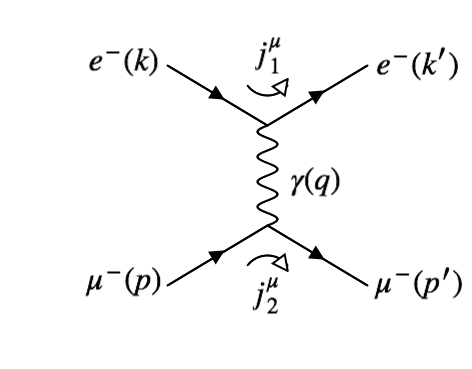
\includegraphics[width=0.5\textwidth]{images/web_feynman/image_87.png}
    \caption[Scattering of electrons and muons with momenta labels]{Scattering of electrons and muons with momenta labels.}
    \label{fig:ch8_EMuToEMuMomenta}
  \end{center}
\end{figure}

The transition amplitude is then:

\begin{eqnarray*}
  T_{fi} & = & -i\int j^{1}_{\mu}\left(\frac{-1}{q^2}\right)j^{\mu}_2 \mathrm{d}^4x \\
  & = & i\e\int\mathrm{d}^4x\bar{u}(k')\e^{ik'x}\gamma_{\mu}u(k)\e^{-ikx}\left(\frac{-1}{q^2}\right)\left(-\e\right)\bar{u}(p')e^{ip'x}\gamma^{\mu}u(p)\e^{-ipx} \\
  & = & \frac{i\e^2}{q^2}\int\mathrm{d}^4x\e^{i\left(k'+p'-k-p\right)}
        \Big[\bar{u}\left(k'\right)\gamma_{\mu}u\left(k\right)\Big]
        \Big[\bar{u}\left(p'\right)\gamma^{\mu}u\left(p\right)\Big]
\end{eqnarray*}

As before for $|T_{fi}|^2$, one exponential term becomes the phase-space factor and the second becomes the product of the volume and time.

\[
  |T_{fi}|^2 = \frac{\e^4}{q^4}
      \Big[\bar{u}\left(k'\right)\gamma_{\mu}u\left(k\right)\Big]
      \Big[\bar{u}\left(p'\right)\gamma^{\mu}u\left(p\right)\Big]
      \Big[\bar{u}\left(k'\right)\gamma_{\mu}u\left(k\right)\Big]^{\dagger}
      \Big[\bar{u}\left(p'\right)\gamma^{\mu}u\left(p\right)\Big]^{\dagger}
\]

The Hermitian conjugates are:

\begin{eqnarray*}
  \big(u^{\dagger}(p')\gamma^0\gamma^{\mu}u(p)\big)^{\dagger} & = & u^{\dagger}(p)\gamma^{\mu\dagger}\gamma^{0\dagger}u(p') \\
  & = & u^{\dagger}(p)\gamma^{\mu\dagger}\gamma^0u(p') \\
  & = & -u^{\dagger}(p)\gamma^{\mu}\gamma^0u(p') \\
  & = & u^{\dagger}(p)\gamma^0\gamma^{\mu}u(p') \\
  & = & \bar{u}(p)\gamma^{\mu}u(p')
\end{eqnarray*}

and similarly for the other term.

\[
  \Rightarrow |T_{fi}|^2 = \frac{\e^4}{q^4}
                           \Big[\bar{u}(k')\gamma_{\mu}u(k)\Big]
                           \Big[\bar{u}(k)\gamma_{\nu}u(k')\Big]
                           \Big[\bar{u}(p')\gamma^{\mu}u(p)\Big]
                           \Big[\bar{u}(p)\gamma^{\nu}u(p')\Big]
\]

\begin{eqnarray*}
  \Big[\bar{u}(k')\gamma_{\mu}u(k)\Big]
  \Big[\bar{u}(k)\gamma_{\nu}u(k')\Big]
  & \quad & \textrm{is the electron tensor} \\
  \Big[\bar{u}(p')\gamma_{\mu}u(p)\Big]
  \Big[\bar{u}(p)\gamma_{\nu}u(p')\Big]
  & \quad & \textrm{is the muon tensor}
\end{eqnarray*}

\[
  |T_{fi}|^2 = \frac{\e^4}{q^4} {}^{\e}L_{\mu\nu} {}^{\mu}L^{\mu\nu}
\]

In order to calculate the transition amplitude correctly the amplitude must be summed over all initial states, summed over all final spin states and averaged over all initial spin states:

\[
  ^{\e}L_{\mu\nu} = \frac{1}{2}\sum_{S}\sum_{S'} \bar{u}(k')\gamma_{\mu}u(k)\bar{u}(k)\gamma_{\nu}u(k')
\]

Writing this explicitly in terms of individual matrix elements, $\alpha$, $\beta$, $\gamma$, $\delta$:

\[
  ^{\e}L_{\mu\nu} = \frac{1}{2}\sum_{S}\sum_{S'}\bar{u}(k')_{\alpha}\gamma_{\mu}^{\alpha\beta}u(k)_{\beta}\bar{u}(k)_{\gamma}\gamma_{\nu}^{\gamma\delta}u(k')_{\delta}
\]

where the factor of $1/2$ is due to the averaging over initial spin states.

These values are all elements of tensors, so they can be reordered:

\begin{eqnarray*}
  ^{\e}L_{\mu\nu} & = & \frac{1}{2}\sum_{S}\sum_{S'}u(k')_{\delta}\bar{u}(k')_{\alpha} \left(\gamma_{\mu}^{\alpha\beta}\right)u(k)_{\beta}\bar{u}(k)_{\gamma}\gamma_{\nu}^{\gamma\delta} \\
  & = & \sum_{S}\sum_{S'}\left(\not{k}' + m\right)_{\delta\alpha} \left(\gamma_{\mu}^{\alpha\beta}\right) \left(\not{k} + m\right)_{\beta\gamma}
\end{eqnarray*}

So ${}^{\e}L_{\mu\nu}$ is reduced to the trace of the product of four $4 \times 4$ matrices:

\begin{eqnarray*}
  {}^{\e}L_{\mu\nu} & = & \frac{1}{2}Tr\Big[ \left(\not{k}' + m\right)\left(\gamma_{\mu}\right)\left(\not{k} + m\right)\left(\gamma_{\nu}\right) \Big] \\
  {}_{\mu}L_{\mu\nu} & = & \frac{1}{2}Tr\Big[ \left(\not{p}' + m\right)\left(\gamma_{\mu}\right)\left(\not{p} + m\right)\left(\gamma_{\nu}\right) \Big]
\end{eqnarray*}

Denoting the electron mass by $m$ and the muon mass by $M$ gives:

\begin{eqnarray*}
  |T_{fi}|^2 & = & \frac{\e^4}{q^4}\frac{1}{2}Tr\Big[\left(\not{k}' + m\right)\gamma_{\mu}\left(\not{k} + m\right)\gamma_{\nu}\Big]\frac{1}{2}Tr\Big[\left(\not{p}' + M\right)\gamma^{\mu}\left(\not{p} + M\right)\gamma^{\nu}\Big] \\
  & = & \frac{\e^4}{4q^4}Tr\Big[\left(\not{k}' + m\right)\gamma_{\mu}\left(\not{k}+m\right)\gamma_{\nu}\Big] Tr\Big[\left(\not{p}' + M\right)\gamma^{\mu}\left(\not{p} + M\right)\gamma^{\nu} \Big]
\end{eqnarray*}

The only non-zero terms are terms involving two or four $\gamma$ matrices.  eg $\left(\not{k}'\gamma_{\mu}m\gamma_{\nu}\right) = 0$.

\begin{eqnarray*}
  \textrm{So } |T_{fi}|^2 & = & \frac{\e^4}{4q^4} Tr[\gamma_{\delta}\gamma_{\mu}\gamma_{\sigma}\gamma_{\nu}k'^{\delta}k^{\sigma} + \gamma_{\mu}\gamma_{\nu}m^2]Tr[\gamma^{\delta}\gamma^{\mu}\gamma^{\sigma}\gamma^{\nu}p'_{\delta}p_{\sigma} + \gamma^{\mu}\gamma^{\nu}M^2] \\
  & = & \frac{\e^4}{q^4} \left( \left(g_{\delta\nu}g_{\nu\sigma} - g_{\delta\sigma}g_{\nu\mu} + g_{\delta\mu}g_{\sigma\nu}\right)k'^{\delta}k^{\sigma} + g^{\mu_\nu}m^2\right) \\
      && \times 4 \left( \left(g^{\delta\nu}g^{\nu\sigma} - g^{\delta\sigma}g^{\nu\mu} + g^{\delta\mu}g^{\sigma\nu}\right)p'_{\delta}p_{\sigma} + g_{\mu\nu}M^2\right) \\
  &&\textrm{Multiplying out: }\\
  |T_{fi}|^2 & = & \frac{8\e^4}{q^4}\left( \left(k'\cdot p'\right)\left(k\cdot p\right) + \left(k'\cdot p\right)\left(k\cdot p'\right) - m^2\left(p'\cdot p\right) - M^2\left(k'\cdot k\right) + m^2M^2\right)
\end{eqnarray*}

In the relativistic limit the $m^2$ and $M^2$ terms can be neglected.

\[
  \Rightarrow |T_{fi}|^2 = \frac{8\e^4}{q^4}\left(\left(k'\cdot p'\right)\left(k\cdot p\right) + \left(k'\cdot p\right)\left(k\cdot p\right)\right)
\]

Expressing this in terms of the Mandelstran variables gives:

\begin{eqnarray*}
  s   & =    & \left(k + p\right)^2 \\
      & \sim & 2k\cdot p \\
      & \sim & 2k'\cdot p' \\
  q^2 & =    & t \\
      & =    & \left(k - k'\right)^2 \\
      & =    & \left(p - p'\right)^2 \\
      & \sim & -2k\cdot k' \\
      & \sim &  2p\cdot p' \\
  u   & =    & \left(k - p'\right)^2 \\
      & \sim & -2p'\cdot k \\
      & \sim & -2k'\cdot p \\
  \textrm{So } |T_{fi}|^2 & = & \frac{8\e^4}{t^2}\left(\frac{s}{2}\frac{s}{2} + \left(\frac{-u}{2}\right)\left(\frac{-u}{2}\right)\right) \\
  & = & \frac{2\e^4}{t^2}\left(s^2 + u^2\right) \\
  & = & 2\e^4\left(\frac{s^2 + u^2}{t^2}\right) \\
  \Rightarrow \frac{\mathrm{d}\sigma}{\mathrm{d}\Omega} & = & \frac{1}{64\pi^2s}|T_{fi}|^2 \\
  & = & \frac{\e^4}{32\pi^2s}\left(\frac{s^2 + u^2}{t^2}\right)
\end{eqnarray*}

\section{Cross section for \texorpdfstring{$\e^+\e^- \to \mu^+\mu^-$}{EEToMuMu}}

This cross section can be easily derived from $e \mu \to e \mu$ scattering.  Compare the Feynmann diagrams shown in figure \ref{fig:ch8_EMuToEMuMomenta}.

\begin{figure}[!htb]
  \begin{center}
    \begin{tabular}{cc}
      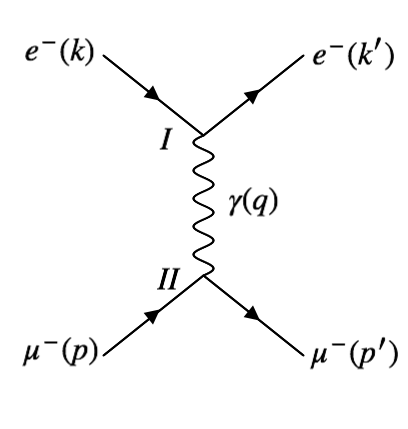
\includegraphics[width=0.4\textwidth]{images/web_feynman/image_25.png} &
      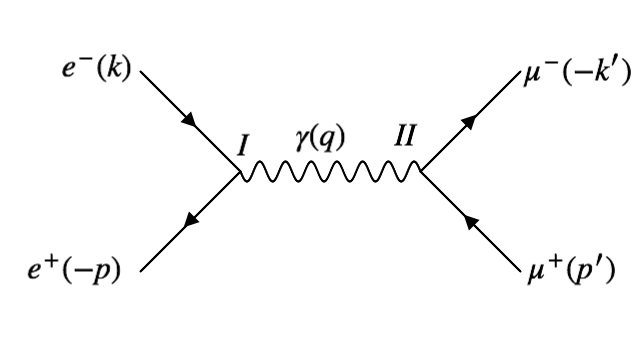
\includegraphics[width=0.6\textwidth]{images/web_feynman/image_26.png}
    \end{tabular}
    \caption[Scattering of electrons and muons with momenta in the $s$ and $t$ channels]{Scattering of electrons and muons with momenta in the $s$ and $t$ channels.}
    \label{fig:ch8_EMuToEMuMomentaSTChannels}
  \end{center}
\end{figure}

Comparing the vertices:

\[
\begin{array}{ccc}
  \textrm{For }I  & k \to k'  & \textrm{in } e\mu \to e\mu         \\
                  & k \to -p  & \textrm{in } e^+e^- \to \mu^+\mu^- \\
  \textrm{For }II & p \to p'  & \textrm{in } e\mu \to e\mu         \\
                  & -k'\to p' & \textrm{in } e^+e^- \to \mu^+\mu^-
\end{array}
\]

So between the two processes there is an interchange of $k'$ with $-p$ and $p$ with $-k'$.

Recall for $e^-\mu^-$ scattering:

\begin{eqnarray*}
  |T_{fi}|^2 & = & \frac{8\e^4}{q^4}\left(\left(k'\cdot p'\right)\left(k\cdot p\right) + \left(k'\cdot p\right)\left(k\cdot p'\right)\right) \\
  \textrm{and } q^4 & = & 4\left(k\cdot k\right)^2 \\
\end{eqnarray*}

So $|T_{fi}|^2$ for $e^+e^-$ is:

\begin{eqnarray*}
  |T_{fi}|^2 & = & \frac{8\e^4}{4\left(k\cdot p\right)^2}\left(\left(p\cdot p'\right)\left(k\cdot k'\right) + \left(p\cdot k'\right)\left(k\cdot p\right)\right) \\
  & = & \frac{2\e^4}{\left(k\cdot p\right)^2}\left(\left(p\cdot p'\right)\left(k\cdot k'\right) + \left(p\cdot k'\right)\left(k\cdot p'\right)\right) \\
  & = & \frac{2\e^4}{\left(\frac{s}{2}\right)^2}\left(\left(\frac{-t}{2}\right)\left(\frac{-t}{2}\right) + \left(\frac{-u}{2}\right)\left(\frac{-u}{2}\right)\right) \\
  \Rightarrow |T_{fi}|^2_{e^+e^-} & = & 2\e^4\left(\frac{t^2 + u^2}{s^2}\right) \\
  \Rightarrow \frac{\mathrm{d}\sigma}{\mathrm{d}\Omega}_{e^+e^-} & = & \frac{1}{64\pi^2}\times2\e^4\left(\frac{t^2 + u^2}{s^2}\right) \\
  & = & \frac{\e^4}{32\pi^2}\left(\frac{t^2 + u^2}{s^2}\right)
\end{eqnarray*}

In comparison with $e\mu \to e\mu$, the values of $s$ and $t$ are simply interchanged.

\subsection{Total cross-section}

To find the total cross-section, integrate with respect to $\Omega$ and evaluate $s$, $t$ and $u$ in terms of the energy and angle of scattering in the centre of mass frame:

\begin{eqnarray*}
  s   & \sim & 2k\cdot p \\
      & =    & 4E_{e^-}E_{e^+} \\
  t^2 & =    & 4\left(k\cdot k'\right)^2 \\
      & =    & 4\left(E_{e^-}E_{\mu^+} - p_{e^-}\cdot p_{\mu^+} \right)^2 \\
      & =    & 4E_{e^-}E_{\mu^+}\left(1 - \cos\theta\right)^2 \\
  u^2 & =    & 4\left(k\cdot p'\right)^2 \\
      & =    & 4E_{e^-}E_{\mu^-}\left(1 + \cos\theta\right)^2 \\
  \Rightarrow \frac{\mathrm{d}\sigma}{\mathrm{d}\Omega} & = & \frac{1}{64\pi^2s}2\e^4\frac{4\left(E_{e^-}E_{\mu^+}\left(1 - \cos\theta\right)^2 + E_{e^-}E_{\mu^-}\left(1 + \cos\theta\right)^2\right)}{16 E_{e^+}E_{e^-}}
\end{eqnarray*}

But in the centre of mass system:

\[
  E_{e^-} = E_{e^+} = E_{\mu^-} = E_{\mu^+}
\]

\begin{eqnarray*}
  \Rightarrow \frac{\mathrm{d}\sigma}{\mathrm{d}\Omega} & = & \frac{1}{64\pi^2s}\e^4\left(1 + \cos\theta\right)^2 \\
  \sigma & = & \int_{-\pi}^{\pi}\frac{\mathrm{d}\sigma}{\mathrm{d}\Omega}\mathrm{d}\Omega \\
  \mathrm{d}\Omega & = & 2\pi \mathrm{d}\left(\cos\theta\right) \\
  \alpha & = & \frac{\e^2}{4\pi} \\
  \Rightarrow \sigma & = & \int_0^{\pi}\frac{\alpha^2}{4s}\left(1 + \cos^2\theta\right) 2\pi\mathrm{d}\left(\cos\theta\right) \\
  & = & \frac{2\pi\alpha^2}{4s}\int_{1}^{-1}\left(1 + x^2\right)\mathrm{d}x \\
  \left(\textrm{as } x \right.& = &\left. \cos\theta\right) \\
  & = & \frac{2\pi\alpha^2}{4s}\Big[-\cos\theta - \frac{1}{3}\cos^3\theta\Big]_0^{\pi} \\
  & = & \frac{4\pi\alpha^2}{3s}
\end{eqnarray*}

The annihilation process falls off as a function of $1/s$.  Had it not been for $q\bar{q}$ resonances, eg $Z^0$, particle physics would have become rather uninteresting.

Note that using similar methods it is possible to calculate Bhabha scattering:

\begin{figure}[!htb]
  \begin{center}
    \begin{tabular}{cc}
      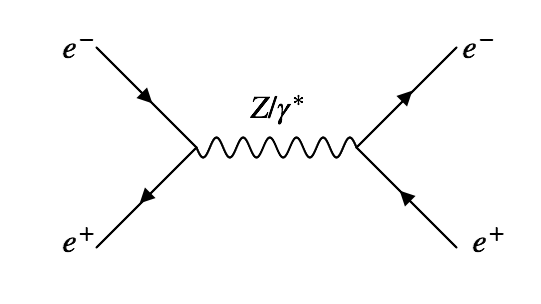
\includegraphics[width=0.5\textwidth]{images/web_feynman/image_28.png} &
      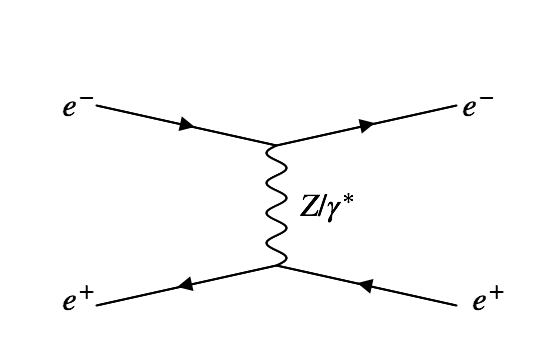
\includegraphics[width=0.5\textwidth]{images/web_feynman/image_29.png}
    \end{tabular}
    \caption[Lowest order Bhabha scattering processes]{Lowest order Bhabha scattering processes.}
    \label{fig:ch8_Bhabha}
  \end{center}
\end{figure}

There are higher order interactions which have not been taken into account, such as:

\begin{figure}[!htb]
  \begin{center}
    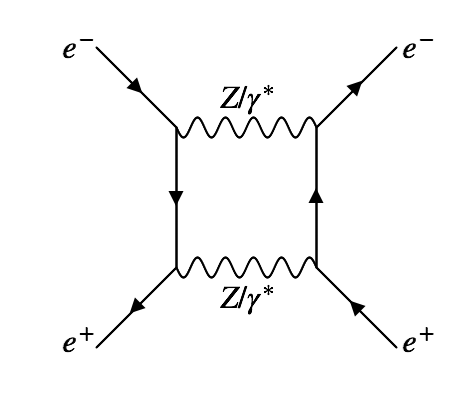
\includegraphics[width=0.5\textwidth]{images/web_feynman/image_30.png}
    \caption[Higher order Bhabha scattering processes]{Higher order Bhabha scattering processes.}
    \label{fig:ch8_Bhabha2}
  \end{center}
\end{figure}

\section{The ratio \texorpdfstring{$R$ at $\e^+\e^-$}{RAtEE} colliders}

\[
  R = \frac{\sigma(e^+e^- \to hadrons)}{\sigma(e^+e^- \to \mu^+\mu^-)}
\]

At low energies $e^+e^-$ can annihilate into systems containing $u$ or $d$ quarks with quarks subsequently hadronising.  They can annihilate through the virtual photon to make $q\bar{q}$ resonances such as the $\rho(770)$.  As the energy increases $s\bar{s}$, $c\bar{c}$ and $b\bar{b}$ states can be formed.  At very high energies $t\bar{t}$ states can be formed, although such $e^+e^-$ colliders have yet to be built.

Consider the contribution to $R$ from on generation of $q\bar{q}$ pairs:

\begin{eqnarray*}
  R & = & \frac{\left(\left(\frac{2}{3}\right)^2 + \left(\frac{-1}{3}\right)^2\right)\times\e^2\times 3}{\e^2} \\
  & = & \frac{15}{9} \textrm{ per generation}
\end{eqnarray*}

By the time the energy is $\sqrt{s}>2m_b$, $R$ should be be $\sim \frac{11}{3}$.

Superimposed are the resonances, such as the $J/\psi$ and $\Upsilon$ family.  There are resonances at $\rho(770)$, $J/\psi(3088)$ and $\Upsilon(10588)$.  At Babar, the $e^+e^-$ collider runs at the $\Upsilon(4S)$ resonances, which decays almost exclusively to $b\bar{b}$ pairs.

\begin{figure}[!htb]
  \begin{center}
    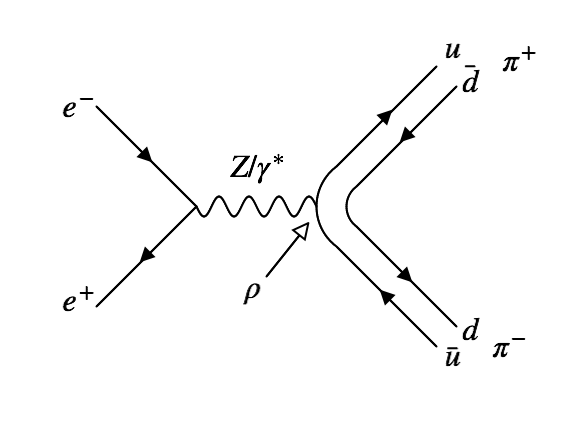
\includegraphics[width=0.5\textwidth]{images/web_feynman/image_31.png}
    \caption[Hadron production ($e^+e^-\to\pi\pi$)]{Hadron production, ($e^+e^-\to\pi\pi$), with a resonant contribution.}
    \label{fig:ch8_EpEmToPiPi}
  \end{center}
\end{figure}

Although the simple model predicting $\frac{11}{3}$ for $R$ for $\sqrt{s}>2m_b$ gives a reasonable description of the data, this is not the complete picture.  The actual value is somewhat higher due to gluon radiation in the final state of the hadronic system:

\begin{figure}[!htb]
  \begin{center}
    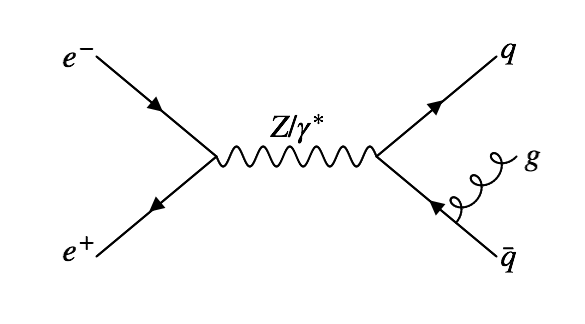
\includegraphics[width=0.5\textwidth]{images/web_feynman/image_32.png}
    \caption[Hadron production with gluon radiation]{Hadron production with gluon radiation.}
    \label{fig:ch8_EpEmToQQG}
  \end{center}
\end{figure}

So there is a higher order correction to $R\sim\frac{11}{3}$.

\begin{figure}[!htb]
  \begin{center}
    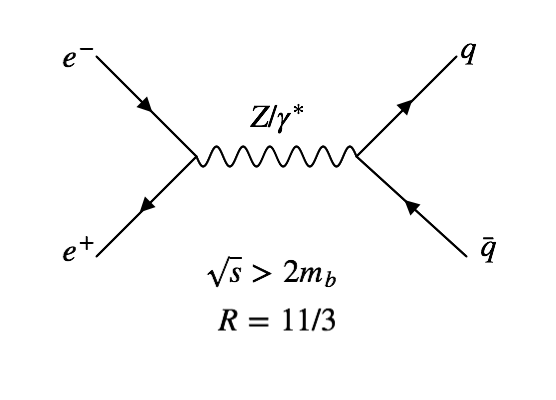
\includegraphics[width=0.5\textwidth]{images/web_feynman/image_34.png}
    \caption[Hadron production and $R$ for $\sqrt{s}>2m_b$]{Hadron production and $R$ for $\sqrt{s}>2m_b$.}
    \label{fig:ch8_EpEmR}
  \end{center}
\end{figure}

At the $Z^0$ mass resonance, an analogous quantity is the ratio of the partial decay widths:

\[
  R_Z = \frac{\Gamma(Z^0 \to hadrons)}{\Gamma(Z^0 \to \mu^+ \mu^-)}
\]

To lowest order, $R_Z = 20.09$, however the measured value is $20.79 \pm 0.04$.  This $3.5\%$ discrepency is due entirely to higher order QCD corrections and gives a good way to measure $\alpha_s$.

\section{Helicity conservation at high energies}

It is possible to gain further insight into cross-section calculations and their angular distributions by looking at the helicity of particles.  The states are:

\begin{eqnarray*}
  U_L & = & \frac{1}{2}\left(1 - \gamma^5\right)u \\
  U_R & = & \frac{1}{2}\left(1 + \gamma^5\right)u \\
  \bar{U}_L & = & U_L^{\dagger}\gamma^0 \\
  & = & \frac{1}{2}\left(U^{\dagger}\right)\left(1 - \gamma^5\right)^{\dagger}\gamma^0 \\
  & = & \frac{1}{2}U^{\dagger}\left(1 - \gamma^5\right)\gamma^0 \\
  & = & \frac{1}{2}U^{\dagger}\gamma^0\left(1 + \gamma^5\right) \\
  & = & \frac{1}{2}\bar{U}\left(1 + \gamma^5\right)
\end{eqnarray*}

At high energies the electromagnetic interaction conserves helicity.

Consider the electromagnetic current:

\begin{eqnarray*}
  \bar{u}\gamma^{\mu}u & = & \left(\bar{U}_L + \bar{U}_R\right)\gamma^{\mu}\left(U_L + U_R\right) \\
  \bar{U}_L\gamma^{\mu}U_R & = & \frac{1}{2}\bar{u}\left(1 + \gamma^5\right)\gamma^{\mu}\frac{1}{2}\left(1 + \gamma^5\right)u \\
  & = & \frac{1}{4}\bar{u}\gamma^{\mu}\left(1 - \gamma^5\right)\left(1 + \gamma^5\right)u \\
  & = & \frac{1}{4}\bar{u}\gamma^{\mu}\left(1 - \left(\gamma^5\right)^2\right)u \\
  & = & 0
\end{eqnarray*}

Helicity conservation requires that the incoming electron and positron have opposite helicities, as do the outgoing muons.

In the centre of mass system:

\begin{figure}[!htb]
  \begin{center}
    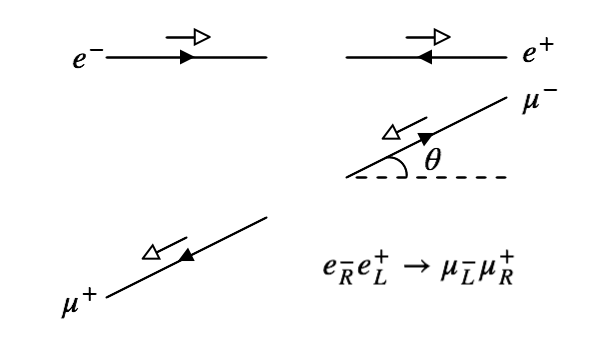
\includegraphics[width=0.75\textwidth]{images/web_feynman/image_33.png}
    \caption[Helicity conservation in a centre of mass system]{Helicity conservation in a centre of mass system.}
    \label{fig:ch8_helicityConservation}
  \end{center}
\end{figure}

The reaction proceeds via a photon of spin$-1$ so the amplitudes are proportional to the rotation matrices:

\[
  d^j_{\lambda\lambda'}(\theta) = \langle j\lambda'|e^{-i\theta J_y}|j \lambda\rangle
\]

where $y$ is perpendicular to the reaction plane.  The rotation matrices can be calculated using angular momentum theory.

\[
  \begin{array}{ccccccc}
  d^1_{1,1}  (\theta) & = & d^1_{-1,-1}(\theta) & = & \frac{1}{2}\left(1 + \cos\theta\right) & \sim & -\frac{u}{s} \\
  d^1_{1,-1} (\theta) & = & d^1_{-1,1} (\theta) & = & \frac{1}{2}\left(1 - \cos\theta\right) & \sim & -\frac{t}{s}
  \end{array}
\]

Squaring and adding the above:

\[
  \frac{\mathrm{d}\sigma}{\mathrm{d}\Omega} \propto \frac{t^2 + u^2}{s^2}
\]
